
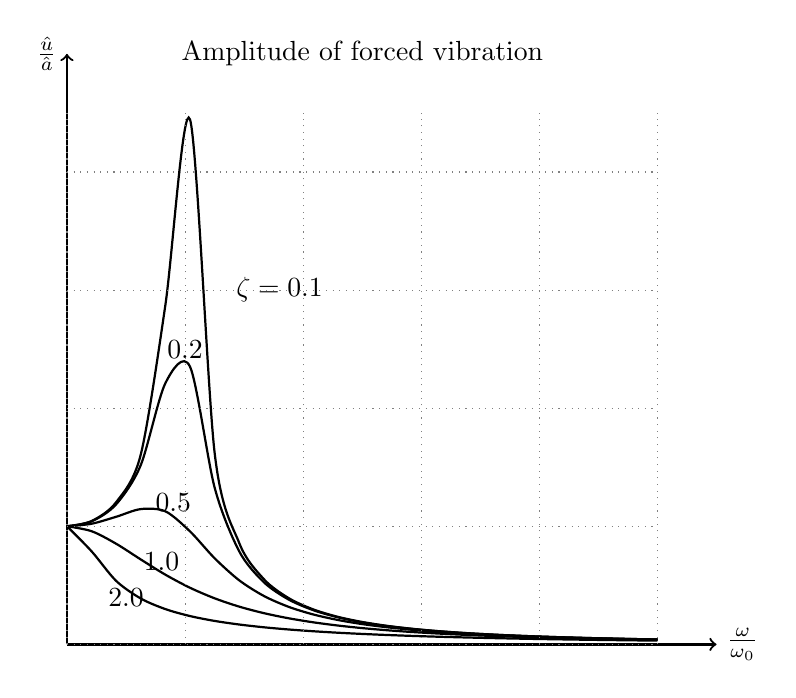
\begin{tikzpicture}[scale=1.5]
    \draw[->, black, thick] (0,0) -- (5.5,0) node[right] {$\frac{\omega}{\omega_0}$};
    \draw[->, black, thick] (0,0) -- (0, 5) node[left] {$\frac{\hat{u}}{\hat{a}}$};
    

    \draw[domain = 0:5, color = black, thick] plot[smooth] (\x,{1 / sqrt((1-\x^2)^2 + (2*0.1*\x)^2)}) node at (1.8, 3) {$\zeta = 0.1$};
    \draw[domain = 0:5, color = black, thick] plot[smooth] (\x, {1 / sqrt((1-\x^2)^2 + (2*0.2*\x)^2)}) node at (1, 2.5) {$0.2$};
    \draw[domain = 0:5, color = black, thick] plot[smooth] (\x, {1 / sqrt((1-\x^2)^2 + (2*0.5*\x)^2)}) node at (0.9, 1.2) {$0.5$};
    \draw[domain = 0:5, color = black, thick] plot[smooth] (\x, {1 / sqrt((1-\x^2)^2 + (2*1.0*\x)^2)}) node at (0.8, 0.7) {$1.0$};
    \draw[domain = 0:5, color = black, thick] plot[smooth] (\x, {1 / sqrt((1-\x^2)^2 + (2*2.0*\x)^2)}) node at (0.5, 0.4) {$2.0$};
    
    %Grid
    \draw[gray, dotted] grid (5,4.5);
    
    \node at (2.5, 5) {Amplitude of forced vibration};
\end{tikzpicture}